\makeheading{Week 8}
\section*{Pit Stop: \emph{Effects} vs. \emph{Terms} in a Linear Predictor}
\textbf{Example}: Suppose \textcolor{Red}{Factor A} has $ m_1=5 $ levels, \textcolor{Orange}{Factor B} has $ m_2=2 $ levels,
and \textcolor{Blue}{Factor C} has $ m_3=3 $ levels.
\begin{itemize}
      \item The main effect for a given factor is represented by indicator variables corresponding to the levels of
            that factor.
            \begin{itemize}
                  \item \textbf{Factor A} will be represented in a regression model by $ m_1-1=4 $ indicator variables: \textcolor{Red}{$ x_1,x_2,x_3,x_4 $},
                        and $ m_1-1=4 $ corresponding $ \beta $'s: \textcolor{Red}{$ \beta_1=\beta_2=\beta_3=\beta_4 $}.
                  \item Thus, the \emph{main effect} of Factor A is composed of 4 \emph{terms} in the model.
                  \item To determine the significance of the main effect of Factor A, we test:
                        \begin{tightcenter}
                              \textcolor{Red}{$\HN$: $\beta_1=\beta_2=\beta_3=\beta_4=0$}.
                        \end{tightcenter}
                  \item \textbf{Factor B} will be represented in a regression model by $ m_2-1=1 $ indicator variable: \textcolor{Orange}{$ x_5 $},
                        and $ m_2-1=1 $ corresponding $ \beta $: \textcolor{Orange}{$ \beta_5 $}.
                  \item Thus, the \emph{main effect} of Factor B is composed of 1 \emph{term} in the model.
                  \item To determine the significance of the main effect of Factor B, we test:
                        \begin{tightcenter}
                              \textcolor{Orange}{$\HN$: $\beta_5=0$}.
                        \end{tightcenter}
                  \item \textbf{Factor C} will be represented in a regression model by $ m_3-1=2 $ indicator variables: \textcolor{Blue}{$ x_6,x_7 $},
                        and $ m_3-1=2 $ corresponding $ \beta $'s: \textcolor{Blue}{$ \beta_6,\beta_7 $}.
                  \item Thus, the \emph{main effect} of Factor C is composed of 2 \emph{terms} in the model.
                  \item To determine the significance of the main effect of Factor C, we test:
                        \begin{tightcenter}
                              \textcolor{Blue}{$\HN$: $\beta_6=\beta_7=0$}.
                        \end{tightcenter}
                  \item \textbf{Note}: These three hypotheses are relevant only in the context of the \emph{main effect} model which has linear predictor:
                        \[ \beta_0+\beta_1x_1+\beta_2x_2+\beta_3x_3+\beta_4x_4+\beta_5x_5+\beta_6x_6+\beta_7x_7 \]
            \end{itemize}
      \item The interaction effect between \emph{two} factors is represented by two-way products of the indicator variables
            corresponding to the main effects of the two factors.
            \begin{itemize}
                  \item The \textbf{A:B interaction} \emph{effect} is composed of the $ (m_1-1)\times (m_2-1)=4\times 1=4 $ \emph{terms}
                        resulting from the two-way products between Factor A's and Factor B's indicator variables: \textcolor{DeepPink}{$ x_1x_5,x_2x_5,x_3x_5,x_4x_5 $},
                        with corresponding $ \beta $'s: \textcolor{DeepPink}{$ \beta_8,\beta_9,\beta_{10},\beta_{11} $}.
                  \item The significance of the A:B interaction effect is determined by testing:
                        \begin{tightcenter}
                              \textcolor{DeepPink}{$ \HN $: $ \beta_8=\beta_9=\beta_{10}=\beta_{11}=0 $}.
                        \end{tightcenter}
                  \item The \textbf{A:C interaction} \emph{effect} is composed of the $ (m_1-1)\times (m_3-1)=4\times 2=8 $ \emph{terms}
                        resulting from the two-way products between Factor A's and Factor C's indicator variables:
                        \[ \textcolor{Indigo}{x_1x_6,x_2x_6,x_3x_6,x_4x_6,x_1x_7,x_2x_7,x_3x_7,x_4x_7}, \]
                        with corresponding $ \beta $'s: \textcolor{Indigo}{$ \beta_{12},\beta_{13},\ldots,\beta_{19} $}.
                  \item The significance of the A:C interaction effect is determined by testing:
                        \begin{tightcenter}
                              \textcolor{Indigo}{$ \HN $: $\beta_{12}=\beta_{13}=\beta_{14}=\beta_{15}=\beta_{16}=\beta_{17}=\beta_{18}=\beta_{19}=0$}.
                        \end{tightcenter}
                  \item The \textbf{B:C interaction} \emph{effect} is composed of the $ (m_2-1)\times (m_3-1)=1\times 2=2 $ \emph{terms}
                        resulting from the two-way products between Factor B's and Factor C's indicator variables: \textcolor{Green}{$ x_5x_6,x_5x_7 $},
                        with corresponding $ \beta $'s: \textcolor{Green}{$ \beta_{20},\beta_{21} $}.
                  \item The significance of the B:C interaction effect is determined by testing:
                        \begin{tightcenter}
                              \textcolor{Green}{$ \HN $: $\beta_{20}=\beta_{21}=0$}.
                        \end{tightcenter}
            \end{itemize}
      \item The interaction effect between \emph{three} factors is represented by three-way products of the indicator variables
            corresponding to the main effects of the three factors.
            \begin{itemize}
                  \item The \textbf{A:B:C interaction} \emph{effect} is composed of the $ (m_1-1)\times (m_2-1)\times (m_3-1)=4\times 1\times 2=8 $ \emph{terms}
                        resulting from the three-way products between Factor A's, Factor B's, and Factor C's indicator variables:
                        \[ \textcolor{Brown}{x_1x_5x_6,x_1x_5x_7,x_2x_5x_6,x_2x_5x_7,x_3x_5x_6,x_3x_5x_7,x_4x_5x_6,x_4x_5x_7}, \]
                        with corresponding $ \beta $'s: \textcolor{Brown}{$ \beta_{22},\ldots,\beta_{29} $}.
                  \item The significance of the A:B:C interaction effect is determined by testing:
                        \begin{tightcenter}
                              \textcolor{Brown}{$ \HN $: $ \beta_{22}=\beta_{23}=\beta_{24}=\beta_{25}=\beta_{26}=\beta_{27}=\beta_{28}=\beta_{29}=0 $}.
                        \end{tightcenter}
                  \item \textbf{Note}: The hypotheses concerning the significance of interaction effects are relevant only in the
                        context of the \emph{full model} which has linear predictor:
                        \begin{align*}
                              \text{Intercept} & \to\beta_{0}+                                                                          \\
                              \text{ME's}      & \to\beta_{1}x_{1}+\beta_{2}x_2+\beta_3x_3+\beta_4x_4+\beta_5x_5+\beta_6x_6+\beta_7x_7+ \\
                              \text{2FI's}     & \to\left\{\begin{array}{l}
                                    \beta_{8}x_1x_5+\beta_9x_2x_5+\beta_{10}x_3x_5+\beta_{11}x_4x_5+\beta_{12}x_1x_6+\beta_{13}x_2x_6+\beta_{14}x_3x_6+ \\
                                    \beta_{15}x_4x_6+\beta_{16}x_1x_7+\beta_{17}x_2x_7+\beta_{18}x_3x_7+\beta_{19}x_4x_7+\beta_{20}x_5x_6+\beta_{21}x_5x_7+
                              \end{array}\right.                                             \\
                              \text{3FI's}     & \to\left\{\begin{array}{l}
                                    \beta_{22}x_1x_5x_6+\beta_{23}x_1x_5x_7+\beta_{24}x_2x_5x_6+\beta_{25}x_2x_5x_7+ \\
                                    \beta_{26}x_3x_5x_6+\beta_{27}x_3x_5x_7+\beta_{28}x_4x_5x_6+\beta_{29}x_4x_5x_7
                              \end{array}\right.                                             \\
                        \end{align*}
            \end{itemize}
      \item \textbf{ALL} the tests discussed here are carried by either a \textbf{partial $\symbf{F}$-test} or a \textbf{likelihood ratio test}.
            \begin{itemize}
                  \item Partial $ F $-test: $ p\text{-value}=\Prob*{T\ge t} $ where $ T \sim F(\nu,h) $.
                  \item Likelihood ratio test: $ p\text{-value}=\Prob*{T\ge t} $ where $ T \sim \chi^2(\nu) $.
                  \item $ \nu=(\text{{\small\#} $\beta$'s in ``full'' model})-(\text{{\small\#} $\beta$'s in ``reduced'' model}) $.
                  \item $ h=\text{error degrees of freedom in the ``full'' model}=N-\text{{\small\#} $\beta$'s in ``full'' model} $.
            \end{itemize}
\end{itemize}
TinyCo is a mobile video game studio that develops the Tiny Zoo game. In this game users own zoos and
collect animals to put in their zoos. An experiment is performed in which a new animal, the
``\href{https://static.wikia.nocookie.net/tinyzoo/images/a/a2/Bananimal_single.png/revision/latest/scale-to-width-down/164?cb=20120325211649}{bananimal},''
is released for purchase as a part of the \href{https://tinyzoo.fandom.com/wiki/Super_Sweet}{Super Sweet Series}. Interest lies in understanding the relationship
between conversion (purchase rate) and two factors: the bananimal’s colour (yellow or gold) and the bananimal's
price ($\$10$, $\$20$, or $\$30$ of in-game currency). A factorial experiment with 6 conditions was performed
to investigate these relationships. A summary of the data resulting from this experiment is shown below.
\begin{table}[!htbp]
      \centering
      \begin{NiceTabular}{|ccc|}
            \toprule
            Condition & Sample Size & Purchase Rate\\
            \midrule
            $ \$10+\text{Yellow} $ & $ 500 $ & $ 0.1720 $\\
            $ \$20+\text{Yellow} $ & $ 483 $ & $ 0.0973 $\\
            $ \$30+\text{Yellow} $ & $ 488 $ & $ 0.0492 $\\
            $ \$10+\text{Gold} $ & $ 500 $ & $ 0.2260 $\\
            $ \$20+\text{Gold} $ & $ 500 $ & $ 0.1840 $\\
            $ \$30+\text{Gold} $ & $ 487 $ & $ 0.1992 $\\
            \bottomrule
      \end{NiceTabular}
\end{table}
\begin{figure}[!htbp]
      \centering
      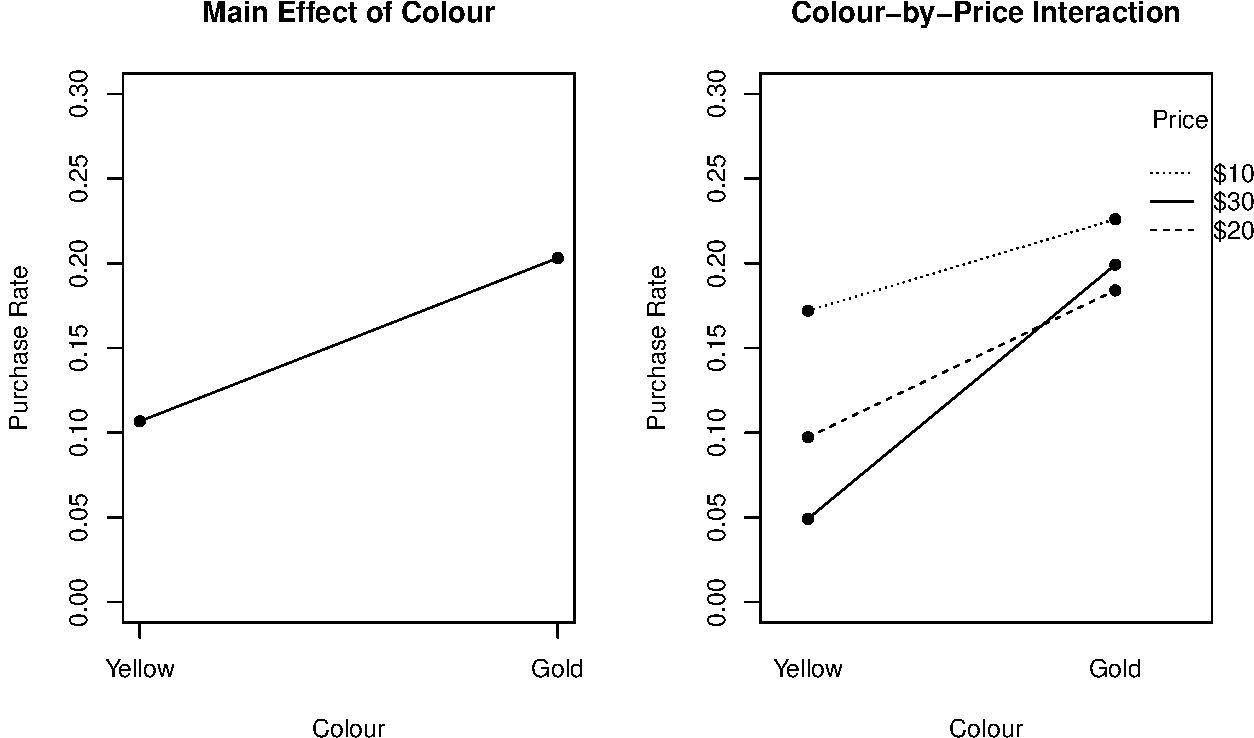
\includegraphics[width=\textwidth]{wk81.pdf}
      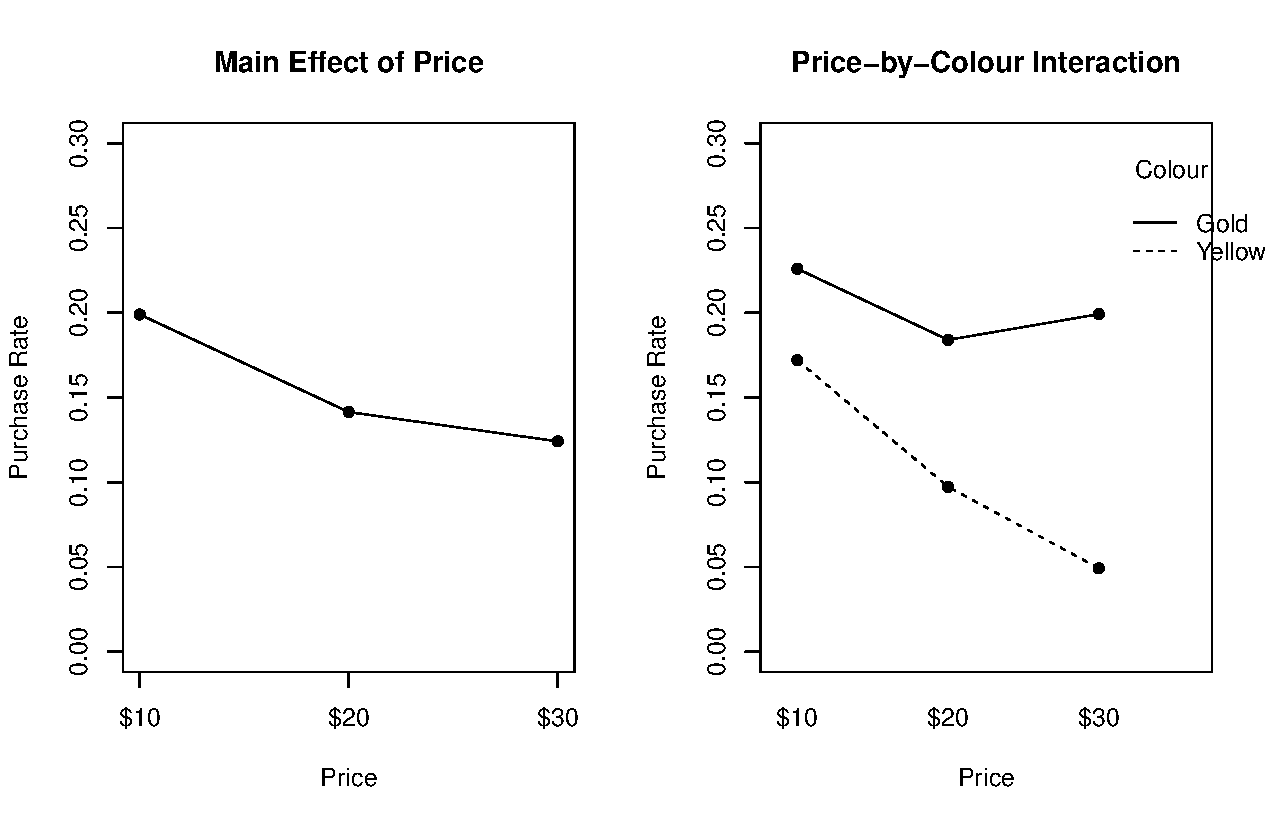
\includegraphics[width=\textwidth]{wk82.pdf}
\end{figure}
\begin{itemize}
      \item What does the main effect plots tell us?
            \begin{itemize}
                  \item ME of colour: gold bananimals are purchased more frequently than yellow.
                  \item ME of price: we expect purchase rate to decrease as bananimal price increases.
                  \item However, we should not stop here because an interaction exists.
            \end{itemize}
      \item What does the interaction effect plots tell us?
            \begin{itemize}
                  \item A price-colour interaction exists.
                  \item We see that increasing price from $ \$20 $ to $ \$30 $ for gold bananimals increases purchase rate,
                        whereas the same increase for yellow bananimals decreases purchase rate.
            \end{itemize}
      \item To formally analyze the data, we fit the \emph{full} logistic regression model with linear predictor:
            \[ \beta_0+{\color{Goldenrod}\beta_1x_{i1}}+{\color{DarkBlue}\beta_2x_{i2}+\beta_3x_{i3}}+{\color{ForestGreen}\beta_4x_{i1}x_{i2}+\beta_5x_{i1}x_{i3}} \]
            \begin{itemize}
                  \item $ x_{i1}=1 $ if unit $ i $ is in a gold bananimal condition.
                  \item $ x_{i2}=1 $ if unit $ i $ is in a $ \$20 $ bananimal condition.
                  \item $ x_{i3}=1 $ if unit $ i $ is in a $ \$30 $ bananimal condition.
            \end{itemize}
      \item We test the significance of the interaction effects via the hypothesis:
            \begin{tightcenter}
                  {\color{ForestGreen}$ \HN $: $ \beta_4=\beta_5=0 $ vs. $ \HA $: $ \beta_j\ne 0 $ for some $ j=4,5 $.}
            \end{tightcenter}
      \item This involves a comparison between the full model and the reduced \emph{main effects} model with linear predictor:
            \[ \beta_0+{\color{Goldenrod}\beta_1x_{i1}}+{\color{DarkBlue}\beta_2x_{i2}+\beta_3x_{i3}} \]
            \begin{itemize}
                  \item $ p\text{-value}=\Prob{T\ge 19.918}=4.731\times 10^{-5} $ where $ T \sim \chi^2(2) $.
                  \item Therefore, we reject $ \HN $ and conclude that the price-colour interaction is significant.
            \end{itemize}
      \item We can also test the main effect of colour with {\color{Goldenrod}$ \HN $: $ \beta_1=0 $} in the context of the main effects model:
            \begin{itemize}
                  \item $ t=53.757 $.
                  \item $ p\text{-value}=2.269\times 10^{-13} $.
                  \item Therefore, we reject $ \HN $ and conclude that colour \underline{does} significantly influence purchase rate.
            \end{itemize}
      \item We can also test the main effect of price with {\color{DarkBlue}$ \HN $: $ \beta_2=\beta_3=0 $} in the context of the main effects model:
            \begin{itemize}
                  \item $ t=23.324 $.
                  \item $ p\text{-value}=8.614\times 10^{-6} $.
                  \item Therefore, we reject $ \HN $ and conclude that price \underline{does} significantly influence purchase rate.
            \end{itemize}
      \item So what have we learned about the influence of these factors?
            \begin{itemize}
                  \item Colour and price both significantly influence purchase rate.
                  \item Gold bananimals tend to be purchased more often than yellow.
                  \item Increasing price from $ \$10 $ to $ \$20 $ decreases purchase rate (for both colours)
                        and increasing price from $ \$20 $ to $ \$30 $ increase purchase rate for gold but not yellow bananimal.
            \end{itemize}
      \item And which condition was optimal?
            \begin{itemize}
                  \item It turns out that the purchase rate is not statistically significantly different in
                        the three gold bananimal conditions. So, $ \$30 $ gold bananimals seem like a good choice for TinyCo.
            \end{itemize}
\end{itemize}
\section*{A Very Brief Introduction to Two-Level Designs}
\begin{itemize}
      \item Factorial experiments are the most informative means of exploring several design factors.
      \item But this may require a larger number of experimental conditions than is practically feasible.
      \item As a compromise, we might consider \textbf{two-level factorial experiments}.
            \begin{itemize}
                  \item This is a factorial experiment where each factor is experimented at just two levels.
            \end{itemize}
      \item Such an experiment is typically used for \textbf{factor screening}.
            \begin{itemize}
                  \item Among a larger number of factors, we want to determine which significantly influence the response.
            \end{itemize}
      \item Factoring screening is predicated on the \textbf{Pareto Principle}.
            \begin{itemize}
                  \item Only a ``vital few'' factors will be important relative to the ``trivial many.''
            \end{itemize}
      \item We will discuss two types of two-level factorial experiments:
            \begin{itemize}
                  \item $ \symbf{2^K} $ \textbf{factorial designs}: investigates $ K $ design factors in $ 2^K $ conditions (i.e., all possible combinations of the factors' levels).
                  \item $ \symbf{2^{K-p}} $ \textbf{factorial designs}: investigates $ K $ design factors in $ 2^{K-p} $ conditions (i.e., just a \underline{fraction} of all possible
                        combinations of the factors' levels).
            \end{itemize}
\end{itemize}
